\documentclass[aspectratio=169]{beamer}

\usepackage{amsmath}
\usepackage{graphicx}
\usepackage{hyperref}
\usepackage{booktabs}
\usepackage{listings}

\lstdefinestyle{pandas}{
  basicstyle=\ttfamily\tiny,
  breaklines=true,
  frame=none,
  backgroundcolor=\color{white},
}

\usetheme{Madrid}
\usecolortheme{seagull}

% Enable frame breaks for long content
\setbeamertemplate{continue label}{}

\title{Coupon Usage Prediction Model}
\subtitle{Machine Learning for Customer Transaction Analysis}
\author{Name Goes Here}
\institute{University Goes Here}
\date{\today}

\begin{document}

\section{Introduction}

\frame{\titlepage}

\begin{frame}{Problem Statement}
\textbf{Research Question:} Do transaction patterns and discount behaviors predict coupon usage?

\textbf{Goal:} Improve coupon targeting and reduce marketing waste

\textbf{Target Variable:} 
\begin{itemize}
    \item \texttt{coupon\_used} (1 = used, 0 = not used) - derived from coupon usage records
\end{itemize}

\textbf{Problem Type:} Binary classification
\begin{itemize}
    \item Features: transaction amounts, customer behavior, time patterns
    \item Response: whether a customer will use a coupon in a transaction
\end{itemize}
\end{frame}

\section{Data Description}

\begin{frame}{Data Description}
\textbf{Data Sources:}
\begin{table}
\centering
\begin{tabular}{lrr}
\toprule
Dataset & Records & Description \\
\midrule
Wallet Transactions & 490,942 & Customer purchases \\
Coupon Usage & 75,676 & Coupons actually used \\
Coupon Distribution & 211,712 & Coupons sent to customers \\
\bottomrule
\end{tabular}
\end{table}

\textbf{Key Patterns to Explore:}
\begin{itemize}
    \item Relationship between transaction amount and coupon usage
    \item Impact of discount depth on redemption rates
    \item Time-based patterns (hour, day of week)
    \item Customer behavior history as predictor
\end{itemize}
\end{frame}

\begin{frame}{Variable Types}
\begin{columns}
\begin{column}{0.5\textwidth}
\textbf{Numeric (8):}
\begin{itemize}
    \item \texttt{tran\_amt}, \texttt{discounts\_amt}, \texttt{point\_amt}
    \item \texttt{coupon\_used\_count}, \texttt{total\_coupon\_used\_amt}
    \item \texttt{coupon\_send\_count}, \texttt{total\_coupon\_send\_amt}
    \item \texttt{benefit\_ratio}, \texttt{discount\_ratio}, \texttt{savings\_pct}
\end{itemize}
\end{column}
\begin{column}{0.5\textwidth}
\textbf{Categorical (5):}
\begin{itemize}
    \item \texttt{station\_code}
    \item \texttt{attributionorgcode}
    \item \texttt{transactionorgcode}
    \item \texttt{hour}, \texttt{day\_of\_week}
    \item \texttt{is\_weekend}, \texttt{is\_morning}
\end{itemize}
\end{column}
\end{columns}

\textbf{Target Variable:} \texttt{coupon\_used} (Binary: 1 = Used, 0 = Not Used)
\end{frame}

\begin{frame}{Sample Data: Raw Input (Pandas)}
\bigskip
\bigskip
\begin{block}{Code}
\texttt{df = pd.read\_csv('cust\_wallet\_detail\_train.csv')}\\
\texttt{df = df.merge(coupon\_used\_agg, on='membercode', how='left')}\\
\texttt{df = df.merge(coupon\_send\_agg, on='membercode', how='left')}
\end{block}
\bigskip
\begin{block}{pd.head(5) - Raw Data (Merged)}
\lstset{style=pandas}
\lstinputlisting[language=Python,firstline=0,lastline=5]{../images/pandas_raw_head.txt}
\end{block}
\end{frame}

\begin{frame}{Sample Data: Processed Features (Pandas)}
\bigskip
\bigskip
\begin{block}{pd.head(5) - Processed Data}
\lstset{style=pandas}
\lstinputlisting[language=Python,firstline=0,lastline=5]{../images/pandas_processed_head.txt}
\end{block}
\end{frame}

\begin{frame}{Key Libraries}
\begin{itemize}
    \item \textbf{pandas}: Data manipulation and analysis
    \item \textbf{numpy}: Numerical computations
    \item \textbf{sklearn}: Machine learning models and evaluation
    \item \textbf{tensorflow}: Neural network implementation
    \item \textbf{ matplotlib}, \textbf{seaborn}: Data visualization
\end{itemize}
\end{frame}

\begin{frame}{Key Functions}
\begin{columns}
\begin{column}{0.5\textwidth}
\textbf{Data Processing:}
\begin{itemize}
    \item \texttt{pd.read\_csv()}: Load datasets
    \item \texttt{df.merge()}: Join datasets
    \item \texttt{df.drop()}: Remove columns
    \item \texttt{df.quantile()}: Outlier removal
\end{itemize}
\end{column}
\begin{column}{0.5\textwidth}
\textbf{Modeling:}
\begin{itemize}
    \item \texttt{GradientBoostingClassifier()}: Build model
    \item \texttt{cross\_val\_score()}: Validate
    \item \texttt{feature\_importances\_}: Get importance
\end{itemize}
\end{column}
\end{columns}
\end{frame}

\begin{frame}{Key Functions (sklearn)}
\begin{columns}
\begin{column}{0.5\textwidth}
\textbf{Data Split:}
\begin{itemize}
    \item \texttt{train\_test\_split()}: Split data (80/20)
    \item \texttt{StratifiedKFold()}: 3-fold CV
    \item \texttt{StandardScaler()}: Feature normalization
\end{itemize}
\bigskip
\textbf{Dimensionality Reduction:}
\begin{itemize}
    \item \texttt{PCA()}: Principal component analysis
    \item \texttt{TSNE()}: t-SNE embedding
    \item \texttt{KernelDensity()}: Density estimation
\end{itemize}
\end{column}
\begin{column}{0.5\textwidth}
\textbf{Model Evaluation:}
\begin{itemize}
    \item \texttt{accuracy\_score()}: Accuracy metric
    \item \texttt{roc\_auc\_score()}: AUC metric
    \item \texttt{classification\_report()}: Precision/Recall/F1
    \item \texttt{confusion\_matrix()}: Confusion matrix
    \item \texttt{cross\_val\_score()}: Validation
\end{itemize}
\end{column}
\end{columns}
\end{frame}

\begin{frame}{Key Functions (matplotlib, seaborn, tensorflow)}
\begin{columns}
\begin{column}{0.5\textwidth}
\textbf{Model Training:}
\begin{itemize}
    \item \texttt{RandomForestClassifier()}: Random Forest
    \item \texttt{GradientBoostingClassifier()}: Gradient Boosting
    \item \texttt{SVC()}: Support Vector Machine
    \item \texttt{LogisticRegression()}: Logistic Regression
\end{itemize}
\textbf{Visualization (matplotlib, seaborn):}
\begin{itemize}
    \item \texttt{plt.savefig()}: Save plots
    \item \texttt{sns.heatmap()}: Correlation heatmap
    \item \texttt{ConfusionMatrixDisplay()}: Confusion matrices
\end{itemize}
\end{column}
\begin{column}{0.5\textwidth}
\textbf{Neural Network (tensorflow):}
\begin{itemize}
    \item \texttt{keras.Sequential()}: Build model
    \item \texttt{layers.Dense()}: Dense layers
    \item \texttt{layers.BatchNormalization()}: Batch norm
    \item \texttt{layers.Dropout()}: Dropout
    \item \texttt{model.compile()}: Compile model
    \item \texttt{model.fit()}: Train model
    \item \texttt{model.predict()}: Predictions
\end{itemize}
\end{column}
\end{columns}
\end{frame}

\section{Data Preprocessing}

\begin{frame}[allowframebreaks]{Data Preprocessing}
\textbf{1. Feature Selection (Removed IDs/Hashes):}
\begin{itemize}
    \item \texttt{membercode}, \texttt{order\_no}, \texttt{external\_order\_no}
    \item \texttt{coupon\_code}, \texttt{user\_id}
\end{itemize}

\textbf{2. Outlier Removal (IQR Method):}
\begin{itemize}
    \item Method: Removed values outside 5th-95th percentile (IQR-based)
    \item Applied to: \texttt{tran\_amt}, \texttt{discounts\_amt}, \texttt{point\_amt}
    \item Why: Extreme values distort model training and visualization
    \item Records reduced: 490,942 $\rightarrow$ 421,590 (~14\% removed)
\end{itemize}

\textbf{3. Colinearity Removal:}
\begin{itemize}
    \item \texttt{receivable\_amt} (99\% correlated with \texttt{tran\_amt})
    \item \texttt{net\_amount}, \texttt{total\_benefit} (redundant)
\end{itemize}
\end{frame}

\begin{frame}[allowframebreaks]{Features}
\textbf{Remaining Features (15):}
\begin{itemize}
    \item Transaction: \texttt{tran\_amt}, \texttt{discounts\_amt}, \texttt{point\_amt}
    \item Customer/Store: \texttt{station\_prefix\_encoded}, \texttt{attributionorgcode}, \texttt{transactionorgcode}
    \item Time-based: \texttt{hour}, \texttt{day\_of\_week}, \texttt{is\_weekend}, \texttt{is\_morning}, etc.
    \item Aggregated: \texttt{coupon\_used\_count}, \texttt{total\_coupon\_used\_amt}
    \item \texttt{coupon\_send\_count}, \texttt{total\_coupon\_send\_amt}
\end{itemize}

\textbf{Engineered Features (5):}
\begin{itemize}
    \item \texttt{benefit\_ratio}, \texttt{discount\_ratio}
    \item \texttt{savings\_pct}, \texttt{point\_to\_discount\_ratio}
    \item \texttt{tran\_to\_receivable\_ratio}
\end{itemize}
\end{frame}

\begin{frame}{Feature Selection}
\textbf{Removed Irrelevant Features (IDs and Hashes):}
\begin{itemize}
    \item \texttt{membercode} - Customer ID (hash)
    \item \texttt{order\_no} - Transaction ID (hash, no date pattern)
    \item \texttt{external\_order\_no} - External ID (hash)
    \item \texttt{coupon\_code} - Coupon ID (hash)
    \item \texttt{user\_id} - User ID (hash)
\end{itemize}
\textbf{Impact:} Removing \texttt{membercode} improved accuracy from 64\% to 66\%
\end{frame}

\begin{frame}{Feature Engineering: Station Code}
\textbf{Problem: High-cardinality numeric feature}
\begin{itemize}
    \item \texttt{station\_code}: 18,806 unique values (treated as numeric)
    \item PCA showed it dominated variance (54\% on PC1)
    \item 23.5\% feature importance - but likely overfitting
\end{itemize}
\bigskip
\textbf{Discovery: Extract station prefix}
\begin{itemize}
    \item First 3 digits = store channel/region
    \item Only 19 unique values
    \item Different prefixes show 22-54\% coupon usage rates
\end{itemize}
\bigskip
\textbf{Experiment Results (Random Forest):}
\begin{itemize}
    \item With station\_code: 74.2\% accuracy
    \item Without station\_code: 74.4\% accuracy
    \item With station\_prefix: \textbf{74.6\% accuracy}
\end{itemize}
\bigskip
\textbf{Result:} station\_prefix has lower importance (4.7\%) but improves generalization.
\end{frame}

\section{Visualization}

\begin{frame}{Correlation Matrix Heatmap}
\begin{figure}
\centering
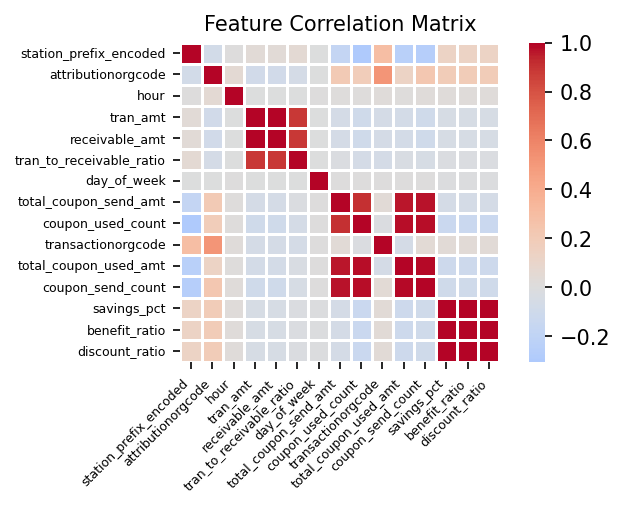
\includegraphics[width=0.7\textwidth]{../images/correlation_matrix.png}
\end{figure}
\end{frame}

\begin{frame}{Density Plot Analysis}
\textbf{Dimensionality Reduction:}
\begin{itemize}
    \item Kernel density estimation (KDE) shows probability distribution
    \item Overlay of two classes on same axes for comparison
    \item X-axis: Transaction amount or Hour, Y-axis: Density
\end{itemize}
\bigskip
\begin{figure}
\centering
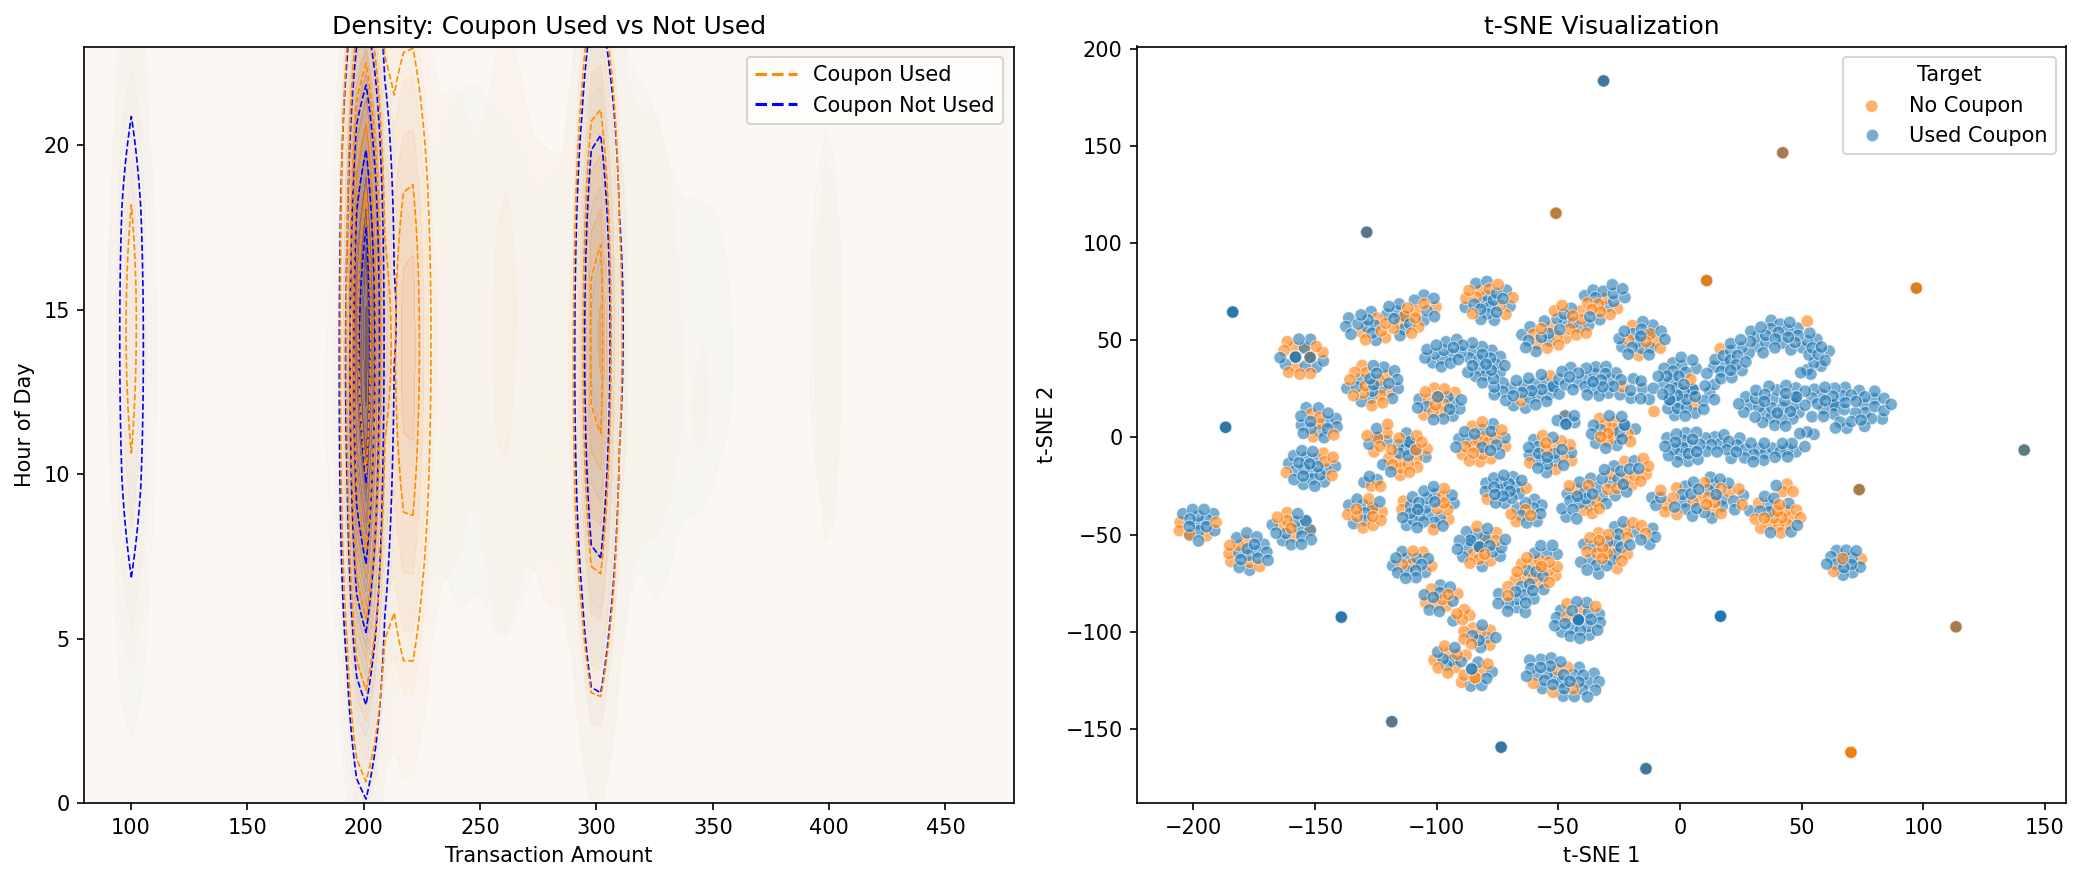
\includegraphics[width=0.8\textwidth]{../images/dimensionality_reduction.png}
\end{figure}
\end{frame}

\begin{frame}{t-SNE Visualization}
\textbf{t-SNE (t-Distributed Stochastic Neighbor Embedding):}
\begin{itemize}
    \item Non-linear dimensionality reduction
    \item Preserves local structure (similar points stay close)
    \item Perplexity=30 used
    \item Reveals class clusters in 2D space
\end{itemize}
\bigskip
\textbf{Key Observations from Density Plot and t-SNE:}
\begin{itemize}
    \item Coupon users (orange) tend to have higher transaction amounts
    \item Non-users (blue) concentrate in lower amounts
    \item Both methods show significant class overlap
    \item No clear linear boundary between classes
    \item Suggests other features needed for better separation
\end{itemize}
\begin{figure}
\centering
%\includegraphics[width=0.7\textwidth]{../images/tsne_visualization.png}
\end{figure}
\end{frame}

\begin{frame}[allowframebreaks]{PCA Visualization}
\begin{columns}
\begin{column}{0.5\textwidth}
\begin{figure}
\centering
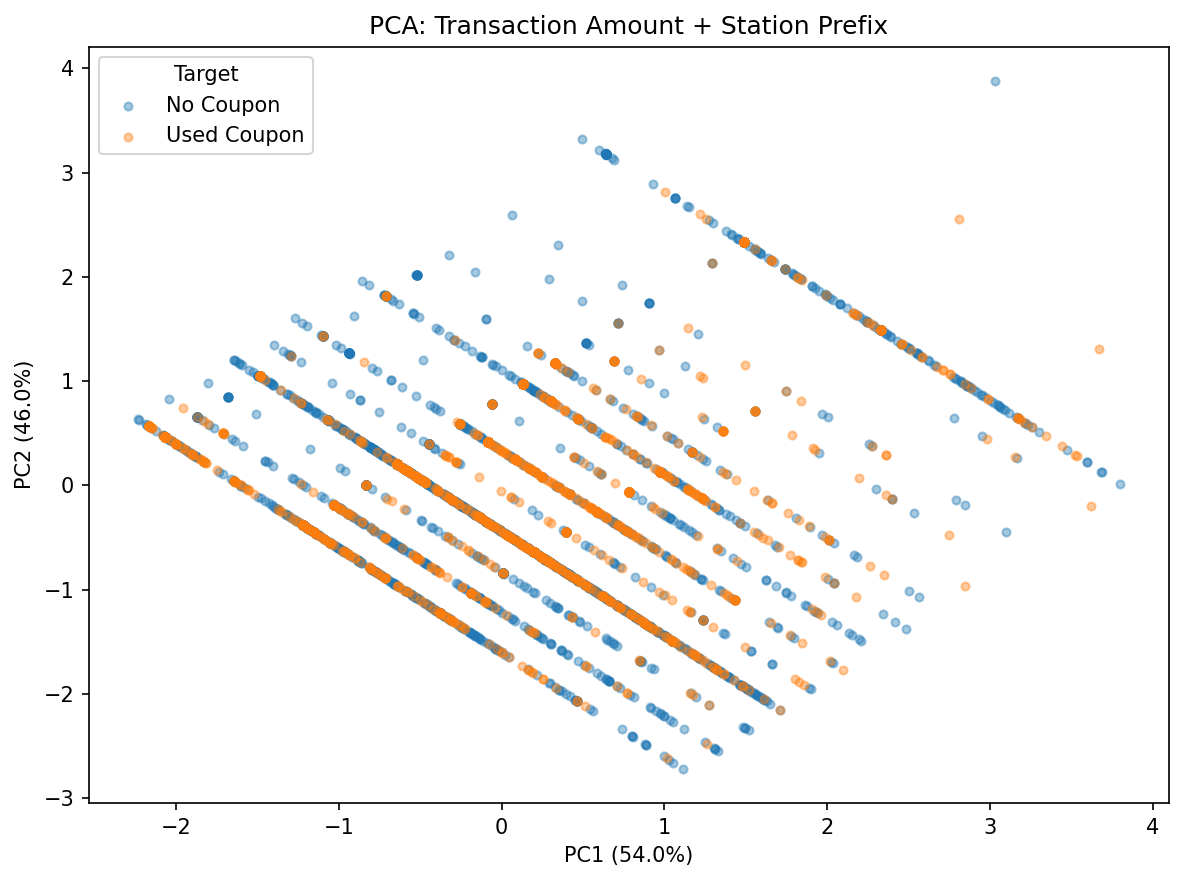
\includegraphics[width=\textwidth]{../images/pca_visualization.png}
\end{figure}
\end{column}
\begin{column}{0.5\textwidth}
\textbf{Key insight: station\_code prefix matters}
\begin{itemize}
    \item Raw station\_code: 18K unique (acts like ID)
    \item Prefix (first 3 digits): 19 unique groups
    \item Prefix shows clear coupon usage patterns:
    \begin{itemize}
        \item 331, 310, 328: ~52\% usage
        \item 334, 335: ~22\% usage
    \end{itemize}
    \item Likely represents store channel/region
\end{itemize}
\end{column}
\end{columns}
\framebreak

\textbf{What the PCA shows:}
\begin{itemize}
    \item Vertical bands = different station prefixes
    \item PC1 (54\%) captures station prefix
    \item PC2 (46\%) captures transaction amount
    \item Within each band: classes overlap significantly
    \item Station prefix is the key differentiator
\end{itemize}
\bigskip
\textbf{Implication for model:}
\begin{itemize}
    \item Feature engineering: extract station prefix
    \item Station/channel is more predictive than transaction amount
\end{itemize}
\end{frame}

\section{Models}

\begin{frame}{Model Architecture}
\begin{columns}
\begin{column}{0.5\textwidth}
\textbf{Random Forest Parameters:}
\begin{itemize}
    \item n\_estimators=100
    \item max\_depth=20
    \item min\_samples\_split=15
    \item min\_samples\_leaf=3
    \item max\_features="sqrt"
\end{itemize}
\bigskip
\textbf{Gradient Boosting Parameters:}
\begin{itemize}
    \item max\_iter=100
    \item max\_depth=10
    \item learning\_rate=0.1
\end{itemize}
\bigskip
\end{column}
\begin{column}{0.5\textwidth}
\textbf{SVM Parameters:}
\begin{itemize}
    \item kernel="rbf"
    \item C=1.0
    \item gamma="scale"
\end{itemize}
\textbf{Logistic Regression Parameters:}
\begin{itemize}
    \item max\_iter=1000
    \item solver="lbfgs"
    \item class\_weight="balanced"
\end{itemize}
\bigskip
\textbf{Data Split: Train/Test: 80/20, Stratified}
\end{column}
\end{columns}
\end{frame}

\begin{frame}{Neural Network Architecture}
\textbf{Neural Network Details:}
\begin{itemize}
    \item Input Layer: 15 features
    \item Hidden Layer 1: 256 neurons (ReLU)
    \item BatchNormalization + Dropout(0.3)
    \item Hidden Layer 2: 128 neurons (ReLU)
    \item BatchNormalization + Dropout(0.3)
    \item Hidden Layer 3: 64 neurons (ReLU)
    \item BatchNormalization + Dropout(0.3)
    \item Output Layer: 2 neurons (Softmax)
\end{itemize}
\textbf{Training:}
\begin{itemize}
    \item Optimizer: Adam (lr=0.001)
    \item Loss: Categorical Crossentropy
    \item Validation Split: 10\%
    \item Batch Size: 256
    \item Epochs: 100
\end{itemize}
\end{frame}

\begin{frame}{Neural Network: Class Weights}
\textbf{Impact of Class Weights on Neural Network:}

\bigskip
\begin{columns}
\begin{column}{0.5\textwidth}
\textbf{Naive (Unbalanced) Weights: \{0:1, 1:2\}}
\begin{itemize}
    \item Accuracy: 62.92\%
    \item Recall: \textbf{92.06\%}
    \item Precision: 49.59\%
    \item Result: Predicts almost everything as positive
\end{itemize}
\end{column}
\begin{column}{0.5\textwidth}
\textbf{Balanced Weights: \{0:1, 1:1\}}
\begin{itemize}
    \item Accuracy: \textbf{71.85\%}
    \item Recall: 58.11\%
    \item Precision: \textbf{62.29\%}
    \item Result: Better balance between precision and recall
\end{itemize}
\end{column}
\end{columns}

\bigskip
Key insight: Naive weights over-predict positives, achieving high recall but low precision. Balanced weights improve overall accuracy and create a more useful model.
\end{frame}

\begin{frame}{Model Performance (20,000 sample)}
\begin{table}
\centering
\begin{tabular}{lrrrrr}
\toprule
Metric & Random Forest & SVM & Gradient Boost & Logistic Reg & Neural Net \\
\midrule
Accuracy & \textbf{74.60\%} & 70.80\% & 73.68\% & 60.48\% & 72.22\% \\
AUC & \textbf{0.825} & 0.761 & 0.818 & 0.676 & 0.799 \\
Precision & 65.40\% & 61.23\% & 63.60\% & 47.20\% & 62.70\% \\
Recall & 64.68\% & 54.69\% & 65.30\% & 69.27\% & 59.14\% \\
F1 Score & \textbf{65.04\%} & 57.77\% & 64.44\% & 56.14\% & 60.87\% \\
\bottomrule
\end{tabular}
\end{table}
Random Forest achieves best accuracy with station\_prefix feature engineering (+0.4\% vs old station\_code).
\end{frame}

\begin{frame}{Sample Size Comparison}
\begin{table}
\centering
\begin{tabular}{lcccc}
\toprule
Model & \shortstack{20,000\\Accuracy} & \shortstack{421,590\\Accuracy} & Improvement \\
\midrule
Random Forest & 74.22\% & \textbf{75.60\%} & +1.38\% \\
Gradient Boosting & 73.62\% & \textbf{74.13\%} & +0.51\% \\
\bottomrule
\end{tabular}
\end{table}
Larger sample size improves model accuracy, with Random Forest showing greater benefit from more data.
\end{frame}

\begin{frame}{Hyperparameter Tuning (Grid Search on Sample Size of 20,000)}
\textbf{Grid Search Results vs Default Parameters:}
\bigskip
\begin{columns}
\begin{column}{0.5\textwidth}
\textbf{Random Forest:}
\begin{itemize}
    \item Best params: max\_depth=10, min\_samples\_leaf=1, n\_estimators=200
    \item Grid Search: 73.80\% accuracy
    \item Default: 74.60\% accuracy
    \item Conclusion: Default params slightly better
\end{itemize}
\end{column}
\begin{column}{0.5\textwidth}
\textbf{Gradient Boosting:}
\begin{itemize}
    \item Best params: learning\_rate=0.1, max\_depth=15
    \item Grid Search: 73.68\% accuracy
    \item Default: 73.68\% accuracy
    \item Conclusion: Similar performance
\end{itemize}
\end{column}
\end{columns}
\end{frame}

\begin{frame}{Hyperparameter Tuning Results (cont.)}
\begin{columns}
\begin{column}{0.5\textwidth}
\textbf{SVM:}
\begin{itemize}
    \item Best params: C=10, gamma='auto'
    \item Grid Search: 71.63\% accuracy
    \item Default: 70.80\% accuracy
    \item Conclusion: +0.8\% improvement
\end{itemize}
\end{column}
\begin{column}{0.5\textwidth}
\textbf{Summary:}
\begin{itemize}
    \item Original parameters were well-tuned
    \item Grid search did not significantly improve results
    \item Random Forest remains best model
    \item Default RF params (74.6\%) $>$ Grid Search (73.8\%)
\end{itemize}
\end{column}
\end{columns}
\end{frame}
\begin{frame}{Grid Search Results Summary}
\begin{table}
\centering
\begin{tabular}{lccc}
\toprule
Model & \shortstack{ROC} & \shortstack{AUC}\\
\midrule
  Random Forest & \textbf{73.80}\% & \textbf{82.02\%}\\
Gradient Boosting & 73.62\% & 81.72\%\\
Support Vecotr Machines & 71.63\% & 77.40 \% \\
\bottomrule
\end{tabular}
\end{table}
  \begin{itemize}
    \item Not a marginal improvement on initial model performance
    \item With more time and resources, hope to expand the grid 
  \end{itemize}
\end{frame}

\begin{frame}{Confusion Matrices}
\begin{figure}
\centering
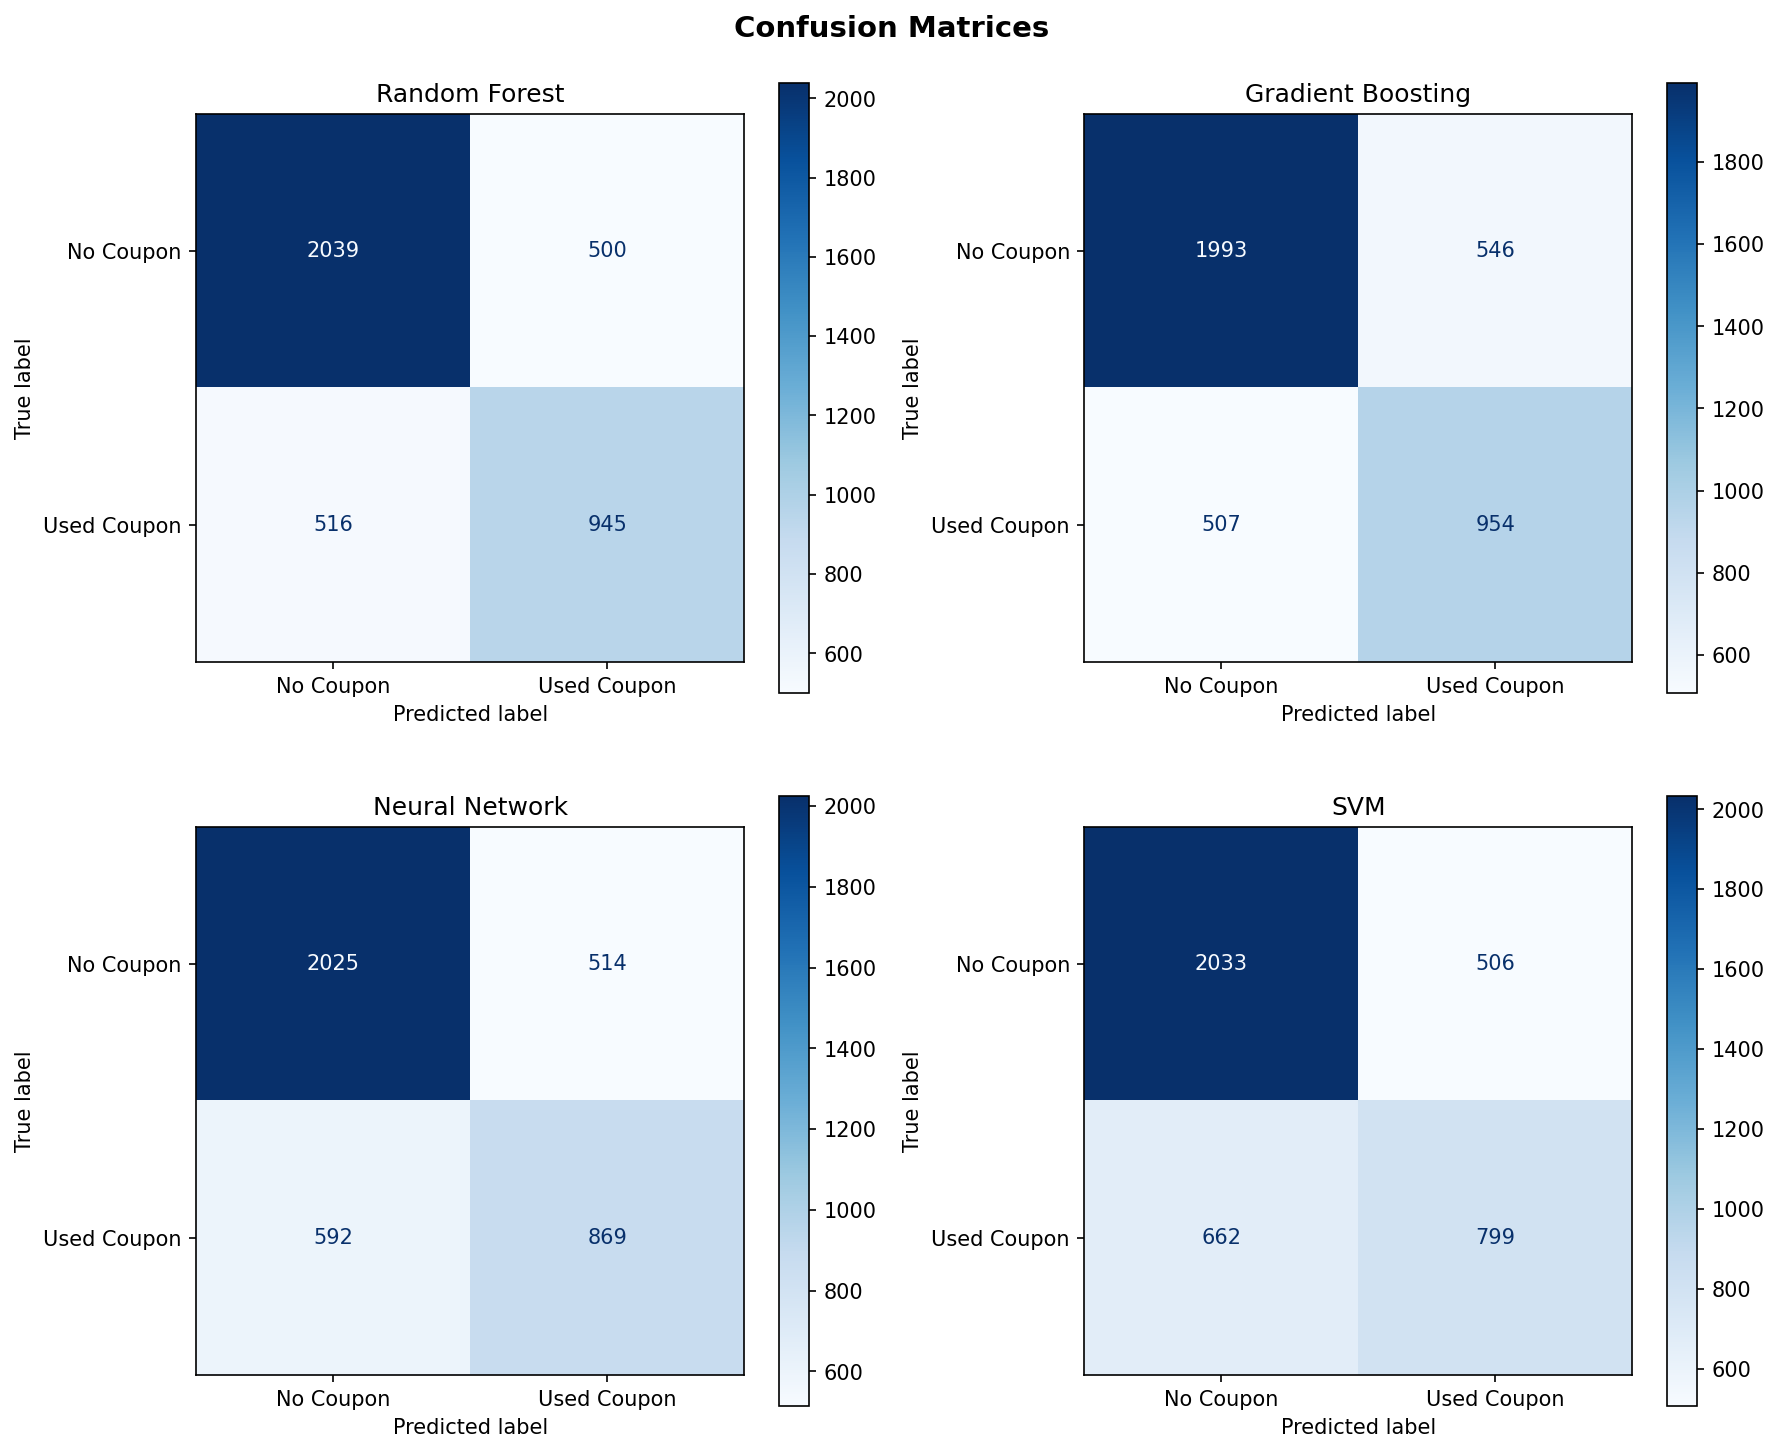
\includegraphics[width=0.9\textwidth,height=0.8\textheight,keepaspectratio]{../images/confusion_matrices.png}
\end{figure}
\end{frame}

\section{Feature Analysis}

\begin{frame}{Feature Importance from Random Forests}
\begin{columns}
\begin{column}{0.5\textwidth}
\begin{figure}
\centering
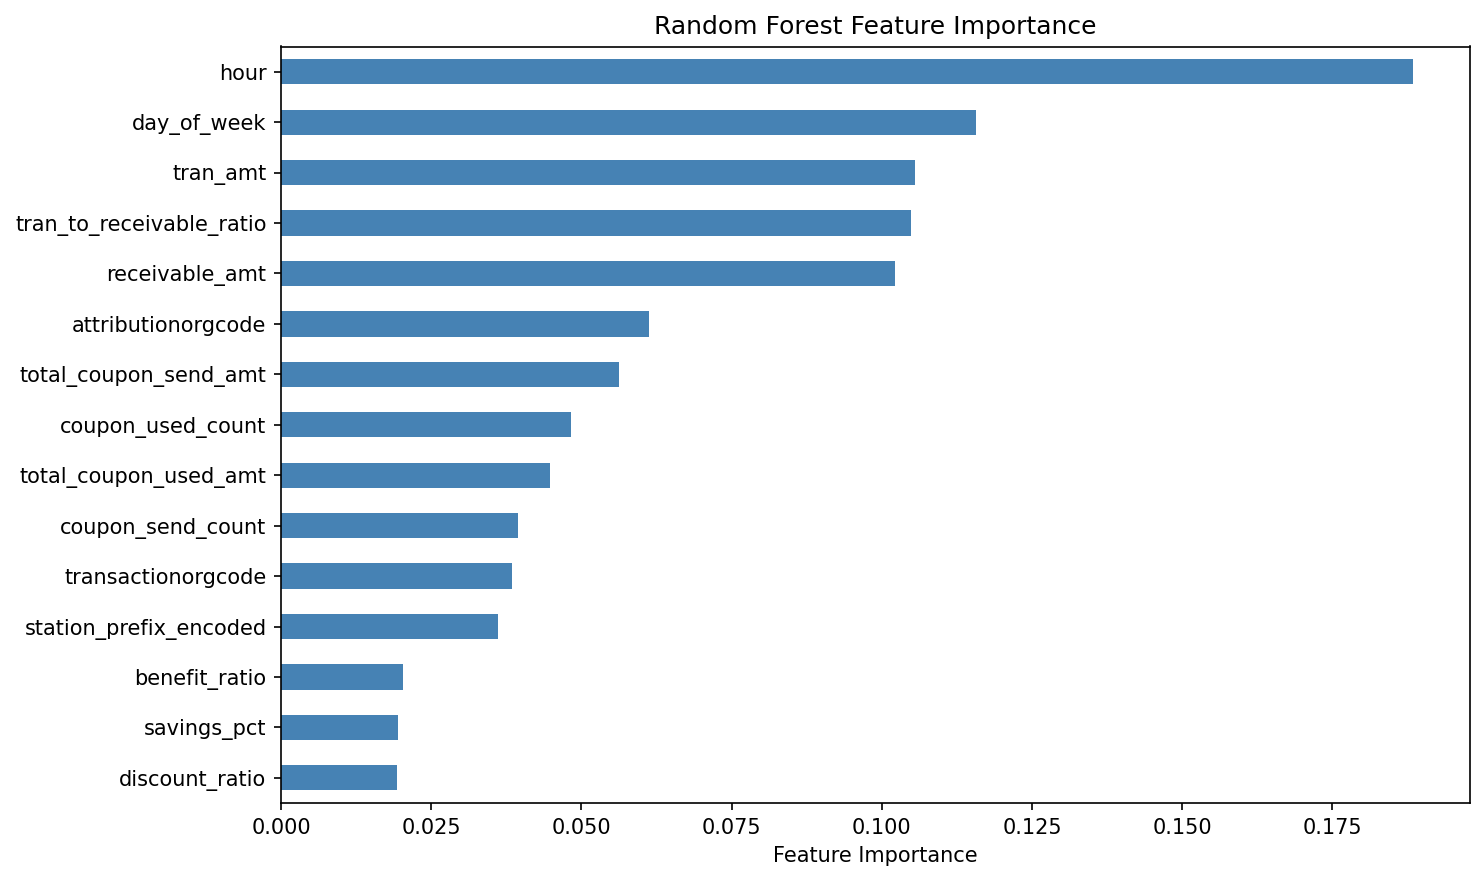
\includegraphics[width=\textwidth]{../images/feature_importance.png}
\end{figure}
\end{column}
\begin{column}{0.5\textwidth}
Top Features:
\begin{enumerate}
    \item \texttt{hour} (15.4\%)
    \item \texttt{tran\_to\_receivable\_ratio} (10.5\%)
    \item \texttt{tran\_amt} (10.5\%)
    \item \texttt{receivable\_amt} (10.2\%)
    \item \texttt{day\_of\_week} (9.3\%)
    \item \texttt{attributionorgcode} (7.5\%)
    \item \texttt{total\_coupon\_send\_amt} (5.4\%)
    \item \texttt{total\_coupon\_used\_amt} (4.9\%)
    \item \texttt{coupon\_used\_count} (4.8\%)
    \item \texttt{coupon\_send\_count} (4.7\%)
    \item \texttt{station\_prefix\_encoded} (4.7\%)
\end{enumerate}
\end{column}
\end{columns}
\end{frame}
\begin{frame}
\textbf{How Feature Importance was Derived:}
\begin{itemize}
    \item Using Random Forest classifier's built-in feature importance
    \item Measures mean decrease in impurity (Gini importance)
    \item Averaged across all 100 decision trees
    \item Higher value = more predictive power
\end{itemize}
\bigskip
\textbf{Key Insight:} Time features (hour, day) and transaction amounts are most predictive. Station prefix has lower feature importance (4.7\%) but improves model generalization (74.6\% accuracy vs 74.2\%).
\end{frame}

\section{Conclusions}

\begin{frame}{Conclusions}
\begin{itemize}
    \item Random Forest achieves \textbf{74.60\% accuracy} with \textbf{0.825 AUC} - best model
    \item Gradient Boosting: 73.68\% accuracy, 0.818 AUC
    \item Neural Network: 72.22\% accuracy with balanced class weights
    \item Feature selection: reduced from 23 to 15 features without accuracy loss
    \item Replaced station\_code with station\_prefix for better generalization
    \item Top features: hour (15.4\%), tran\_to\_receivable\_ratio (10.5\%)
    \item 3-Fold Cross Validation confirms model stability
\end{itemize}
\end{frame}

\begin{frame}{Future Work}
\textbf{Potential Improvements:}
\begin{itemize}
    \item \textbf{Hyperparameter Tuning}: Grid search or random search for optimal parameters. Explore other kernels, $C$ and $\gamma$ sizes for SVM.
    \item \textbf{Advanced Models}: XGBoost, LightGBM for potentially better performance
    \item \textbf{Feature Engineering}: More customer behavior features, time-series patterns
    \item \textbf{Class Imbalance}: Explore SMOTE, undersampling techniques
    \item \textbf{Deployment}: Build API for real-time coupon prediction
\end{itemize}
\end{frame}


\begin{frame}{Repository}
\bigskip
\textbf{GitHub Repository:}\\
\textcolor{blue}{\url{https://github.com/alexanderneva/statscoupons}}\\
\bigskip
\bigskip
All code, data, and presentation materials are available in this repository.
\end{frame}

\end{document}
